\documentclass{hotnets16}

% Comment out the following line to disable comments
\def\commentenabled{1}

\usepackage{times}  
\usepackage{epsfig}
\usepackage[TABBOTCAP]{subfigure}
\usepackage{tabularx}
\usepackage{graphicx} 
\usepackage{color}
\usepackage{xspace}
\usepackage{thumbpdf}
\usepackage{listings}
\usepackage{verbatim}
\usepackage{hyperref}
\usepackage{booktabs}
\usepackage{colortbl}
\usepackage{caption}
\usepackage{todonotes}
\usepackage{mathtools}
\usepackage{amsmath}
\usepackage{cleveref}
\usepackage{eqnarray}

\newtheorem{property}{Property}
\newtheorem{theorem}{Theorem}

\newcommand{\minisection}[1]{\smallskip\noindent{\bf #1.}}
\newcommand{\secref}[1]{{\S\ref{#1}}}
\newcommand{\secsref}[2]{{Sections~\ref{#1} and \S\ref{#2}}}
\newcommand{\figsref}[2]{{Figure~\ref{#1} and \ref{#2}}}
\newcommand{\appref}[1]{{Appendix~\ref{#1}}}
\newcommand{\thmref}[1]{{Theorem~\ref{#1}}}
\newcommand{\lemref}[1]{{Lemma~\ref{#1}}}
\newcommand{\corref}[1]{{Corollary~\ref{#1}}}
\newcommand{\proref}[1]{{Property~\ref{#1}}}

\newcommand{\compactcaption}[1]{\vspace{-1em}\caption{#1}\vspace{-1em}}
\newcommand{\botcompactcaption}[1]{\caption{#1}\vspace{-1em}}
\newcommand{\topcompactcaption}[1]{\vspace{-1em}\caption{#1}\vspace{-0.5em}}

\newenvironment{compactitemize}
{
   \begin{itemize}[leftmargin=1.5em]
   \vspace{-1ex}
   \setlength{\topsep}{0pt}
   \setlength{\itemsep}{0em}
   \setlength{\parskip}{0pt}
   \setlength{\parsep}{0pt}
}
{
   \vspace{-1ex}
   \end{itemize}
}
\newenvironment{compact2itemize}
{
	\begin{itemize}[leftmargin=1.5em]
		\vspace{-1ex}
		\setlength{\topsep}{0pt}
		\setlength{\itemsep}{0.5em}
		\setlength{\parskip}{0pt}
		\setlength{\parsep}{0pt}
	}
	{
		\vspace{-1ex}
	\end{itemize}
}


\newenvironment{compactenumerate}
{
   \begin{enumerate}[leftmargin=1.5em]
   \vspace{-1ex}
   \setlength{\topsep}{0pt}
   \setlength{\itemsep}{0em}
   \setlength{\parskip}{0pt}
   \setlength{\parsep}{0pt}
}
{
   \vspace{-1ex}
   \end{enumerate}
}

\ifdefined\commentenabled
    \newcommand{\loris}[1]{\textcolor[rgb]{0.00,0.00,1.00}{L: #1}}
    \newcommand{\aditya}[1]{\textcolor[rgb]{0.00,0.00,1.00}{A:#1}}
    \newcommand{\kausik}[1]{\textcolor[rgb]{0.2,0.80,0.2}{K: #1}}
    \newcommand{\aaron}[1]{\textcolor[rgb]{0.00,0.2,0.6}{AGJ: #1}}
\else
    \newcommand{\loris}[1]{}
    \newcommand{\aditya}[1]{}
    \newcommand{\kausik}[1]{}
    \newcommand{\aaron}[1]{}
\fi

\newcommand{\ARC}{ARC\xspace}
\newcommand{\ARCs}{ARCs\xspace}


\hypersetup{pdfstartview=FitH,pdfpagelayout=SinglePage}

\setlength\paperheight {11in}
\setlength\paperwidth {8.5in}
\setlength{\textwidth}{7in}
\setlength{\textheight}{9.25in}
\setlength{\oddsidemargin}{-.25in}
\setlength{\evensidemargin}{-.25in}
%\setlength{\headsep}{0in}
%\pagenumbering{arabic}

\begin{document}

\conferenceinfo{HotNets 2016} {}
\CopyrightYear{2016}
\crdata{X}
\date{}

%%%%%%%%%%%% THIS IS WHERE WE PUT IN THE TITLE AND AUTHORS %%%%%%%%%%%%

\title{Policy Enforcement using \\ Distributed Control Plane Synthesis}

\author{Anonymous}

\maketitle

%\thispagestyle{empty}

%%%%%%%%%%%%%  ABSTRACT GOES HERE %%%%%%%%%%%%%%
\subsection*{Abstract}

Synthesizing ARCs ...

\section{Introduction}
%% Conventionally, a network primarily acted as a backbone for
%% communication among machines, and these communications used the
%% ``shortest" path in the network based on certain metrics for deciding
%% the path between two machines.  Today,

Many enterprises are increasingly migrating their on-premise IT
infrastructure to cloud datacenters. In such environments, the
different enterprises (tenants) share different resources, such as,
the compute machines that run their applications and network
infrastructure used for communication among these applications.
Operators of such multi-tenant datacenters thus have to deal with a
multitude of machines communicating with each other (flows) over a
network that is composed of many tens to hundreds of routers or
switches (devices)~\cite{mpa-imc15}. With growing diversity of
enterprise applications and the need for security and compliance,
these pathways of communication through the datacenter network are
subject to increasingly complex network-based policies.

Consider an enterprise tenant in such a datacenter. She may desire
basic communication among her applications along shortest paths based
on certain metrics (reachability). In addition, she may wish that
traffic attempting to reach some of her applications be examined by a
set of ``middleboxes'' for auditing and access control
(traversal). Another tenant may additionally desire a subset of her
flows not share any infrastructure with others' flows for strong
security or Quality-of-Service considerations (isolation).  In
parallel, cloud operators must meet key operational objectives. For
instance, they often need to optimize network performance objectives
(traffic engineering), e.g., minimizing the maximum load imposed by
all tenants on network links, and deal with resource constraints such
as link capacity bounds and switch table sizes. Also, since datacenter
networks are highly prone to link/switch
failures~\cite{datacenterfailures}, operators need to gracefully
transition the old (pre-failure) dataplane to a policy-compliant new
(post-failure) one in a rapid and/or efficient manner.

Today, configuring network devices to implement these complex policies
and objectives in aggregate is manual, ad-hoc, and error-prone.  This
can lead to misconfigurations and violations of tenant service-level
agreements (SLAs) which can have a severe performance and security
impact.

%%  However, in real-life, the
%% process of policy enforcement by network operators is manual and
%% ad-hoc, leading to violations of service-level agreements and
%% mis-configurations which have severe performance and security
%% impacts. With the boom in cloud services, datacenter networks deal
%% with thousands of flows which are not constant, but in flux, thus,
%% making it difficult to enforce them in an ad-hoc manner.

%% Network operators desire various different end-to-end policies to
%% support in clouds and enterprise networks. Tenants or organisations
%% require support for basic policies like reachability between hosts,
%% and specifying different middlebox policies for certain
%% flows. Operators, on top of that require support for complex policies
%% like traffic isolation between flows to provide fairness and
%% specifying resource constraints like link bandwidth and switch table
%% sizes to perform traffic engineering and network resource management.

The rise of \emph{software-defined networking} (SDN) has allowed
operators to program networks in a more intuitive manner. In SDN, a
general-purpose centralized controller machine (control plane)
controls end-to-end communication pathways by managing network
forwarding rules on a collection of programmable switches (data
plane). Using a global view of current network topology, the
controller can program forwarding rules on switches based on
application requirements.
%However, many existing SDN
%frameworks are too low-level, 
%making it challenging 
%to write controller applications using these which generate 
% the data plane enforcing the above policies. %% For many
%% of the policies, generating the data plane is an NP-complete problem
%% and requires the design of efficient custom heuristics; combining
%% different policies' heuristics together is non-trivial.
Unfortunately, existing SDN programming languages (e.g.,
Frenetic~\cite{frenetic} and Pyretic~\cite{pyretic}) are too
constraining: operators would ideally want to specify and realize
policies/objectives network-wide, whereas these languages focus on programming
{\em individual} switch behaviors.  Moreover, for many types of
policies, generating a data plane that enforces them is a
%  an NP-complete 
computationally hard problem, requiring the design of efficient custom
heuristics {\em per policy/objective type}. Other recent works on
network-wide policy enforcement~\cite{merlin,simple} go beyond the
single-switch model, but they target specific types of policies/objectives and
thus are difficult to extend to other commonly desired policy types
(e.g., isolation).
%; combining  different policies' heuristics together is non-trivial. 
 %% \aditya{we need to be
% careful
%%   not to bin all SDN languages into this switch-by-switch model}
%% \kausik{Do you want to make changes here?}







%% support
%% other kinds of policies such as traffic isolation.

%%  like
%% joint bandwidth provisioning and waypoint routing in Merlin
%% \cite{merlin}, and middlebox policy enforcement in SIMPLE
%% \cite{simple} or FlowTags~\cite{flowtags}. However, these approaches

In this paper, we seek a {\em general} approach that allows a variety
of rich policies/objectives to be specified as the input, with the output being
the corresponding set of switch forwarding rules such that the
complexities of correctly realizing the policies in the data plane are
hidden from operators. This is an important step toward {\em
  intent-based networking}~\cite{intent}, where operators specify {\em
  what} they want the network to do instead of worrying about {\em
  how} the network must be configured.
%their networks. %% To support a cornucopia of policies, an
%% important feature is \emph{generality} of the approach of policy
%% enforcement, so that it can be extended to enforce custom policies
%% required by the operator.
This paper makes a case for using \emph{data plane synthesis} as a
practical approach to realizing this vision in the multi-tenant
datacenter context.
%% switch
%% table forwarding rules to the solve the problem of policy enforcement
%% by use of off-the-shelf SMT-solvers.

We present \Name, a framework for {\em declaratively} specifying and
enforcing complex policies and objectives such as, isolation,
middlebox traversals and failure resilience. To tackle the high
complexity of enforcing some of these policies (for e.g., enforcing
isolation is NP-complete), \Name encodes the problem as that of
constraint solving and leverages recent advances in fast
Satisfiability Modulo Theories (SMT) solvers to efficiently search for
a solution to the constraints.  The solution is then translated into
switch forwarding rules.
%Using SMT solvers with 
%support for linear optimization, \name can perform traffic engineering, and
%minimal network repair. We extend \name to synthesize
%resilient switch tables to \emph{proactively} ensure policy-compliance
%in failure scenarios. 
%% This
%% paper presents Genesis, a
%% network management tool where the network operators can express the
%% network-wide policies in a high-level declarative manner and Genesis
%% will synthesize the lower-level switch forwarding rules for realising
%% these policies, eliminating the need for operators to work on
%% switch-level behaviours. 
By leveraging the formal guarantees of constraint solving, \Name
eliminates the room for error in the enforcement of complex
policies and objectives.

%\kausik{Do we need to make the point of sacrificing performance for generality for POPL? }

Unfortunately, due to the the large space of forwarding plane
configurations, naively encoding policies using SMT solvers results in
slow synthesis speeds (up to hundreds-thousands of seconds in the
median case; \secref{sec:baselineeval}) which can be impractical.
%enterprise networks today because the space of forwarding plane configurations
%is huge. 
To make synthesis more practical, \Name leverages domain-specific
properties to simplify the constraints handled by the SMT solver.
We allow the network operator to write restricted
forms of regular expressions, called \emph{tactics}, that blacklist
paths based on certain patterns that are not desired in a datacenter
network.
%\loris{how about: ...based on path patterns that are not desired...}
These tactics are used to discard several constraints, 
acting as a search strategy for the solver.
%\aditya{the previous sentence is vague}
%By identifying a restricted syntax for specifying
%tactics, we 
Tactics can improve the synthesis procedure and achieve
%constraints added to the solver without additional constraints
%required to ensure the solution satisfies the tactic and achieve
a 1.5$\times - $400$\times$ speedup 
(median speedup: 1.6$\times$, average speedup: 22$\times$).

 Secondly, we develop a \emph{divide-and-conquer} synthesis procedure
 that leverages the relationships among  isolation policies to
 improve synthesis performance. The procedure partitions the input
 policies into effective components such that \name can synthesize
 these components separately and faster than the complete problem.
 Divide-and-conquer synthesis can halve the synthesis time for 40\% of
 synthetic isolation workloads.
 %% which vary in size and complexity
 %% of isolation.
 %\aditya{is this statement correct? what is 40\% of scenarios?}
 %\aditya{the
   %previous sentence is vague} 

%% are
%% huge, and by supporting a set of diverse and complex policies with
%% different search objectives, we require to create a model general and
%% expressive enough to support these. This poses a challenge as to can
%% synthesis performance be improved by leveraging knowledge specific to
%% the problem of policy enforcement in networks?

%We implement \Name using ... We evaluate it using .... Key highlights .... \aditya{all of these are todo}.\kausik{Do we need a para or will the next para suffice?}
\noindent \textbf{Contributions.} \ \ \ Our contributions are the following.
\begin{compactitemize}
\item An extensible declarative framework for describing
  complex policies/objectives and a modular SMT-based algorithm for enforcing policies and objectives
  like isolation, waypoints (\secref{sec:synthesisalgo}), traffic engineering~(\secref{sec:optimization}), and 
  failure resiliency (\secref{sec:resiliency});
\item A modified synthesis algorithm based on tactics, which leverages datacenter network structure
  to blacklist undesirable path patterns (\secref{sec:tactic});
\item A divide-and-conquer procedure for speeding up synthesis by leveraging the 
structure of policy interactions (\secref{sec:optimistic});
\item An implementation of \Name and an extensive evaluation on
  different policy/objective workloads, topologies and multi-tenancy
  settings (\secref{sec:evaluation}).
		%to quantify the performance of Genesis. 
\end{compactitemize}
%\aditya{todo}

\iffull\else
A long version
of this paper containing all the proofs has been submitted as supplementary material.
\fi
%% : We present the design and implementation of a network management
%% system with support for a diverse set of complex end-to-end
%% policies like isolation, waypoints and capacity. We designed a
%% novel search strategy using regular expressions to prune the space
%% of forwarding plane configurations by leveraging the network
%% structure to provide properties of the path, especially in
%% datacenter topologies. Lastly, we design a heuristical synthesis
%% routine leveraging the nature of policy interactions to improve
%% synthesis performance.

\section{Vision and Challenges} \label{sec:vision}
% Programming a legacy network control plane to satisfy a variety of
% connectivity, security, and performance policies is a complex and error-prone
% task. We have shown that program synthesis is a promising approach to automate
% this process and produce a control plane that is ``correct-by-construction.''
% In particular, we presented an architecture where a network operator provides
% a policy-compliant data plane and a set of hard and soft policies as input,
% and the system automatically provides a set of device configurations that
% leverage the control plane features available on each device to compute
% policy-compliant paths, even in the presence of failures.  Formulating a
% tractable synthesis problem and maximizing the number of satisfied soft
% policies are the key challenges in realizing this vision. We show these
% challenges can be overcome by modeling the control plane using a graph-based 
% abstract representation tied to a traditional shortest path algorithm and
% iteratively transforming the abstract representation based on feedback from
% the satisfiability (SAT) solver and characteristics of the graph. However, we
% have only explored how to address a subset of important policies and leverage a
% few available control plane features on traditional networking hardware. Our
% future work will focus on satisfying a wider range of policies using more
% features, and we will study how to best translate our abstract representation
% into actual device configurations to make our system practical for use with
% real networks.

One of the foremost tasks in network management is programming the network to
forward traffic in a manner consistent with user- and application-induced
policies. Common types of policies include: reachability (i.e., which
end-hosts can communicate), isolation (i.e., which flows cannot share links),
service chaining (i.e., which middleboxes must be traversed), resilience
(e.g., how many backup paths are available), and traffic engineering. Every
set of forwarding paths (i.e., data plane) installed in the network---either
manually or by a control plane---should conform to these operator-provided
policies, otherwise performance, security, or availability problems may arise.

A variety of techniques can be used to determine the appropriate forwarding
paths. One option is to compute a data plane offline, and install the data
plane using an API that allows direct control of switches' forwarding tables
(e.g., OpenFlow). Several recent works~\cite{merlin, simple} have adopted this
approach, using solvers to automatically compute a data
plane that conforms to a set of policies. \aaron{need to say what is wrong
 with this approach} A second option is to dynamically compute forwarding
paths at a logically centralized controller---i.e., use a software-defined
networking (SDN) control plane. However, this requires developing algorithms
that take the set of policies and the current state of the network (e.g.,
which links have failed) as input and output paths that conform to a
multiplicity of policies.  Most existing SDN control applications only compute
paths based on one or a few types of policies: e.g., service
chaining~\cite{simple, flowtags}, traffic engineering~\cite{swan, b4}, or
resilience~\cite{plinko}. Furthermore, the controller may become bottlenecked
or fail (even if it is distributed), leading to (a partial) network failure.

A third option, which continues to be the most widely adopted, is to
dynamically compute forwarding paths using distributed routing protocols
running on ``legacy'' network switches---i.e., use a ``traditional'' network
control plane. This avoids the scalability, failure tolerance, and \aaron{what
else?} challenges of the other two approaches. However, programming (i.e.,
configuring) a traditional control plane to compute policy-compliant paths
remains challenging for several reasons: (1) the path-computation algorithms
are pre-defined---e.g., OSPF uses Dijkstra's shortest path---and their
behavior can only be influenced through a limited set of parameters---e.g.,
link weights; (2) there is often no direct mapping between policies---e.g.,
isolation---and configuration options---e.g., link weights and route filters;
and (3) a single set of parameters must result in policy-compliant paths under
all possible network states---e.g., all combinations of link failures.
\aaron{Anything else?}

These issues motivate us to design a system that automatically synthesizes
(configurations for) a control plane that computes policy-compliant paths
under all possible network states.
Unfortunately, this task is inherently challenging as it requires solving in one shot multiple
computationally hard problems.
For example, even when considering static routing and no failures, synthesizing a control plane that satisfies  policies such as isolation and waypoints
is an NP-hard problem.
Although the progress in SMT solving has made many NP-hard problems more practical, 
 attempts of incorporating concepts such as shortest path algorithms 
into these solvers have resulted into huge performance losses~\cite{monosat}. 
Finally, adding failure-handling to the problem results in yet another layer of combinatorial explosion.

Our proposed approach is to tackle these three problems in separate phases.
By choosing a data plane as input to the second phase, we 
express the problem of finding a control plane using only the 
theory of linear rational arithmetic (LRA), for which we can use
efficient off-the-shelf LP-solvers. 
This approach causes information to be lost between the different phases;
the data plane generated by the first phase may not be suitable to 
synthesize a control plane conforming to all policies required, and 
the synthesis could fail in the second or third phase. 
However, our architecture can overcome this shortcoming 
by performing
multiple iterations of the first phase to produce different 
candidate data planes for the second and third phases.
Our preliminary results for the three-phase
approach show encouraging performance, and we 
postulate the implementation of 
efficient procedures to enumerate different data 
planes satisfying the input policies for a 
producer-consumer model to make the synthesis of 
control planes from policies tractable.  


The solution space of output network configurations to 
enforce a set of policies
is large; configurations can use different 
network protocols (e.g., only BGP, only OSPF or a hybrid) and
mechanisms (e.g., route filters, access control lists
or protocol-specific variables). The large solution space
of configurations complicates the synthesis of
network configurations from
input policies, 
or ties the synthesis to a particular type of configuration. 
Instead, we borrow a page from programming languages
research and
synthesize an Abstract Representation for Control planes (ARC)~\cite{arc} 
from the data plane; the ARC can then be translated to actual device configurations.
The ARC uses the notion that most routing protocols in use 
today employ a cost-based path selection algorithm; thus a weighted
graph can be used to abstractly represent the control plane such that 
the path between two points taken in the network would be 
the lowest weight path in the graph. 
The ARC effectively decouples the policy component with the 
actual network infrastructure. 

While we use an abstract representation of the control
plane (ARC) to simplify the synthesis, operators need control 
planes conforming to certain requirements of the 
underlying network infrastructure. For example, a 
network may comprise of switches which do not have custom
features like ACLs or route-filters, thus the ARC must take 
into consideration these requirements. Without losing 
generality, we translate these 
requirements as types of ARCs with different properties,
and still use a protocol-independent representation
to represent the control plane. 
% thus, the networking infrastructure could be
% transitioned to different protocols without affecting the policy 
% control of the architecture. From the ARC, we can construct different
% drivers for translation to actual device configurations; these drivers
% can leverage inferences from healthy network practices in 
% real-life networks~\cite{mpa-imc15} to produce ideal network configurations.


%\aaron{Old text below}
%
%To tackle synthesis 
%of distributed control planes, 
%we use as input the network data plane 
%(set of forwarding paths) \aaron{Where does this data plane come from and
%    why is it reasonable to assume an operator can provide one?} which 
%enforces the operator-specified policies to
%synthesize an abstract representation of the control plane
%called ARC. \aaron{Our approach (ARC) should not come up until later in the
%    motivation, if at all.}
%The advantage of using network data planes as 
%input is the ease of developing
%different network management applications 
%enforcing proactive policies\footnote{
%Traditional control planes cannot support reactive policies, however
%middleboxes can overcome this limitation.} 
%as if operating over a software-defined
%network, agnostic of the actual network protocols used in the network.
%\aaron{I don't understand the preceding sentence. I'm still not clear why you
%take a single data plane as input and not multiple data planes or just the
%policies. I realize it is hard to synthesize from the latter, but can you be
%more precise why it is hard?}
%Many existing network management systems like Merlin~\cite{merlin} 
%and SIMPLE~\cite{simple}\footnote{
%Traditional control planes cannot support 
%paths with loops for service chaining.} developed for SDNs 
%could be seamlessly integrated to the architecture with minimal changes.
%\aaron{Do we need the preceding sentence?}
%Thus, using the data plane as input, we synthesize a control plane
%such that the paths decided by the control plane are the same 
%as the data plane input, and these paths satisfy the operator 
%policies.
%
%However, the control plane does not guarantee policy compliance 
%when failures occur. For
%example, if a link along the shortest path 
%%(\aaron{refer to some example figure}) 
%fails, \aaron{Need to mention earlier that we assume shortest-path-based route
%computations, ala OSPF} the next shortest path will become the new path to reach the
%destination. The control plane automatically computes the new shortest path
%(assuming one exists), thus preserving connectivity. 
%However, the new path may
%not conform to the same policies as the path in the 
%original failure-free data
%plane from which the control plane was synthesized: 
%e.g., the new path may no longer
%traverse a waypoint or have the same bandwidth capacity. Thus,
%synthesis must take into account policy-compliance under failures.
%
%Policy-compliance under failures is difficult to achieve due 
%to the large number of failure scenarios to consider and can 
%be impossible to synthesize a control plane which is 
%policy-compliant under all failures. Operators require 
%varying degrees of policy-compliance under failures for 
%which we propose two classes of policies: {\em hard} and
%{\em soft} policies. Operators can specify 
%hard policies pertaining
%to security are of the utmost importance, 
%because they protect the network and
%its services from attacks and unauthorized accesses. Some 
%examples of hard policies are as follows: 
%a particular flow must always traverse through a waypoint 
%under any failure scenario, or a certain pair of hosts must 
%never be able to communicate (always blocked). 
%Soft policies can be considered as objectives which improve 
%the control plane, but are not strict requirements, typically
%pertaining to performance. The consequences of violating
%soft policies are less severe. Operators can provide 
%backup paths for flows (generated such that they 
%satisfy the data plane policies) as soft policies, 
%and the synthesis of the control plane 
%tries to satisfy as many soft policies as 
%possible. 
%
%\aaron{Discussion of the available control plane constructs should come up
%    earlier.}
%While we use an abstract representation of the control
%plane (ARC) to simplify the synthesis, operators need control 
%planes conforming to certain requirements of the 
%underlying network infrastructure. For example, a 
%network may comprise of switches which do not have custom
%features like ACLs or route-filters, thus the ARC must take 
%into consideration these requirements. Without losing 
%generality, we translate these 
%requirements as policies determining the properties of the
%ARC, and thus, still use a protocol-independent representation
%to represent the control plane. 
%
%Our architecture envisions network operator providing
%a policy-compliant data plane and a set of hard and soft policies
%pertaining to policy-compliance under failure and network 
%infrastructure requirements as input to synthesize resilient 
%control planes. Towards this vision, we present  
%approaches to synthesize different types of the ARC and the 
%challenges involved in making synthesis efficient and
%extending these approaches to support a wider range of 
%policies and functionalities. 


% \section{Related Work}
% --- Fill In Later ---
% % Fibbing: Lies can cause loops if the centralized controller fails,
% % our approach is sounder

% <Write about ARC here because people may not have read about it yet>

\section{Synthesis Algorithm} \label{sec:synthesisalgo}
Given a set of policies, \Name creates constraints 
that abstract the forwarding and reachability rules such that the paths
satisfy the input policies.  
These constraints are then given to an SMT Solver, which returns a model 
for them--i.e., it assigns values to all the variables in the constraints. From these values, we extract the forwarding rules for each switch.
To provide support for the policies in \Cref{tab:policysupport}, \name uses propositional logic (SAT), linear rational arithmetic (LRA),
and linear optimization objectives for traffic engineering.
\subsection{Network Forwarding Model} \label{sec:fwdmodel}
We define the physical switch topology as an undirected graph $T=(S, L)$,
where $S$ is the set of switches and $L$ is the set of links. 
We use the neighbour function $N(s) = \{s'\ | \ (s,s') \in L \}$ to denote 
the set of neighbour switches of $s$. 
We define a set of packet classes $PC : [0,\lambda]$ and map each reachability/waypoint policy to a unique integer in $PC$.
The set of reachability policies is denoted as $R$ and each reachability policy $r \in R$ is
a pair
$(predicate :\newline src >> W_1;W_2; \ldots W_n >> dst, pc)$
where:
\begin{compactitemize}
\item  $predicate$ is the packet header identifier pertaining to $r$;
\item  $src,dst \in S$ are the source and destination switches;
\item $W_1, W_2, \ldots, W_n \subseteq S$ are the (potentially empty) ordered sets of waypoints; 
\item $pc \in PC$ is the packet class and is a unique integer used to identify the variables associated to $r$
\end{compactitemize} 
In the rest of the paper, we often use the term packet class to identify the corresponding reachability/waypoint policy. 
Other policies are not mapped to packet classes as they do not produce a path, but specify restrictions on paths of packet classes. 
%Assuming that the intersection of predicates is empty for policies in $R$, we create a mapping $\gamma : R \rightarrow PC$ to associate each reachability policy with a unique integer called packet class in the set $PC$. Switches $src, dst \in S$ denote the ingress and egress switches respectively for the packet class $pc = \gamma(r)$ and Genesis finds a path from $src$ to $dst$ for $pc$. If a waypoint policy is specified, $W$ is the set of switches the path from $src$ to $dst$ must traverse through in no particular order.
We define a static integer $\mu$ to be the synthetic limit for path length for any packet class, and define the set $K = [0, \mu]$ to be the set of all permissible path lengths.

The key roles of the network forwarding model are abstracting the actual forwarding rules at each node and encoding the reachability of each flow. 
\begin{mydef}
\label{def:fwd}
The relation $Fwd \subseteq S \times S \times PC $ captures network forwarding behavior, i.e. 
$(sw_1, sw_2$, $pc)\in$ $Fwd$ if 
$sw_1$ forwards packets of class $pc$ to switch $sw_2$. 
\end{mydef}
\begin{mydef}
\label{def:reach}
	The relation $Reach \subseteq S \times PC \times K$ captures the path reachability,
	i.e. $(sw, pc, k)\in Reach$ if 
	the switch $sw$ is reachable in the path from source switch of packet class $pc$ in exactly $k$ steps.  
\end{mydef}
For brevity, we write $Fwd(sw_1, sw_2, pc)$ for $(sw_1, sw_2, pc) $ $\in Fwd$ and similarly for the $Reach$ relation. 
Since $Fwd$ depends on the topology,
for all $sw_1, sw_2$ that are not connected by a link, 
we have that $\forall pc$, $(sw_1,sw_2,pc) \notin Fwd$. 
\begin{mydef}
	Given the set of constraints $\Psi$ generated by the synthesis algorithm from the input policies,
	$(Fwd,Reach) \models \Psi$ if $Fwd$ and $Reach$ is a model of $\Psi$.
\end{mydef}

\begin{mydef} \label{def:Pi}
Given two concrete relations $Fwd$ and $Reach$, 
the set of induced paths $\Pi = \texttt{paths}(Fwd, Reach)$ is defined as follows:
given a class $pc$,  $(sw_0 \ldots sw_k, pc) \in \Pi$ iff : 
\begin{compactenumerate}
	\item $\forall i \in [0,k]. (sw_i, pc, i) \in Reach$
	\item $\forall i \in [0, k - 1]. (sw_i, sw_{i+1}, pc) \in Fwd$
\end{compactenumerate}
\end{mydef}
\noindent Figure~\ref{fig:model} illustrates these definitions.

\begin{figure}
	\centering
	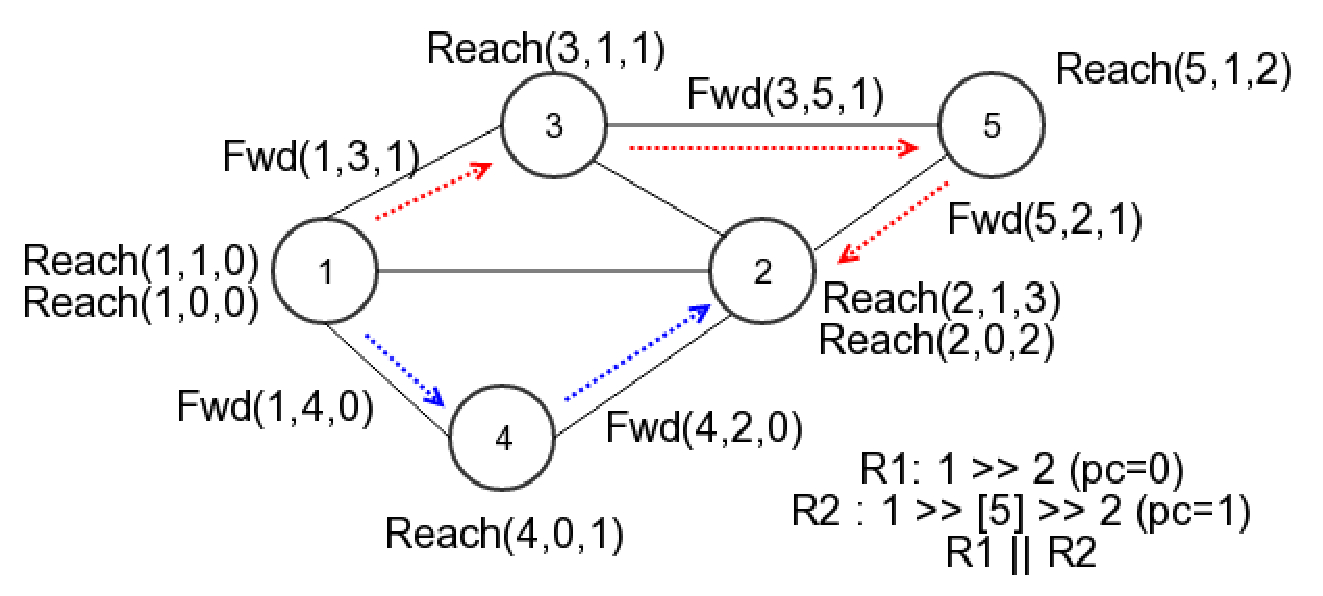
\includegraphics[width=0.8\columnwidth]{figures/network-model-example.eps}
	\caption{Values of the $Fwd$ and $Reach$ relations of the network forwarding model
		 for the policies specified in the figure. The blue and red arrows indicate the 
		 paths of packet classes 0 and 1 respectively according to the model.}
	\label{fig:model}
\end{figure}

\begin{mydef}
Given the set of constraints $\Psi$ corresponding to the input policies,
a set of paths $\Pi$ is a solution to $\Psi$, $\Pi \models \Psi$, 
if there exists $Fwd, Reach$ such that $(Fwd, Reach) \models \Psi$ and $\ \Pi=\texttt{paths}(Fwd,Reach)$.

\end{mydef}
%An example network forwarding model is shown in \cref{fig:model}. 
%%There are two reachability policies, $r1 : 1 >> [5] >> 2$ with $pc=1$ and $r2 : 1 >> 2$ with $pc=2$ and $r1$ is isolated to $r2$
%Using the value of $Fwd$ relation, we can find out paths for each packet class the forwarding rules for each switch. 

One of the decisions oriented towards performance is modelling the forwarding and reachability relations using propositions, so that we can reduce enforcement of policies like reachability, waypoints and isolation to a Boolean Satisfiability Problem (SAT) problem\footnote{An earlier iteration of our model used \emph{uninterpreted functions} and modeled reachability using recursive constraints, 
	which was slower with a greater number of constraints.}. 
The relations for forwarding and reachability ensure we can write the constraints in a concise and intuitive manner.

\subsection{Reachability Constraints} \label{sec:reach}
We first discuss the constraints generated for reachability policies without waypoints.
For a reachability policy $s >> d$ and packet class $pc$, the added constraints must ensure that 
the solution model represents a path 
from source to destination. 
The base constraint states that $(s, pc,0) \in Reach$ meaning
that $s$ can be reached in $0$ steps. 
The following constraint states that there must be a forwarding rule from $s$ to one of
the neighbors of $s$\footnote{
	We unroll the existential quantifier $\exists n \in N(s)$ using disjunction of 
	clauses $\bigvee\limits_{n \in N(s)}$ and
	the universal quantifier $\forall n \in N(dst)$ using conjunction of clauses $\bigwedge\limits_{n \in N(dst)}$
	and stay in propositional logic.}.
\begin{equation} \label{eq:src}
	\exists n \in N(s).~Fwd(s, n, pc) \wedge Reach(n, pc, 1).
\end{equation}
Next, we add the following constraints to state that $d$ can be reached in some number of steps and,
since $d$ is the last switch in the path, there are no forwarding rules from it.
\begin{equation} \label{eq:dst}
	\exists k.~Reach(d, pc, k) \ \wedge \ \forall n \in N(d). \ \neg Fwd(d, n, pc).
\end{equation}
Finally, we add implication constraints that propagate reachability backward from destination to source. 
If a node $n_1$ is reachable in $k$ steps, there must be a node $n_2$ reachable in  $k-1$ steps and 
a forwarding rule $n_2 \rightarrow n_1$.
\begin{multline} \label{eq:bckprop}
\forall n_1,k.~ Reach(n_1,pc,k) \implies \exists n_2.  n_2 \in N(n_1) \wedge \\ Reach(n_2,pc,k-1) \wedge Fwd(n_2,n_1,pc).
\end{multline} 
When combined together, these constraints %can only be satisfied if there is a valid path from $s$ to $d$.
% to destination by using the unit clauses in \cref{eq:dst}, and finding a path from destination back to a switch $sw$ which is a neighbour of $src$. $Reach(sw,pc,1)$ would be true from \cref{eq:src} and the reachability policy would be satisfied. 
are sufficient to ensure the existence of a path from $s$ to $d$ for packet class $pc$.
% in terms of the forwarding relation $Fwd$. 
However, since there is no restriction on number of $Fwd$ values that can be true at a switch, we can get multiple forwarding rules at switches, and 
also multiple paths to the destination. 
These can also create forwarding loops. 
Concretely, this is not a problem: as long as there is  at least one path from $s$ to $d$ we can recover it from the solution of the constraints. 
Moreover, this representation is quite efficient, as forcing a singular path would
require to add further constraints.
% we are able to extract a path from the solution without 
%adding additional constraints to ensure the semantics of \emph{unicast} forwarding. 

To extract a concrete $s$-to-$d$ path we 
perform a breadth-first search on the reachability graph induced by the solution to the constraints. 
A directed edge $n_1 \rightarrow n_2$ appears in the reachability-graph if there is forwarding rule indicated by the relation $(n_1,n_2, pc) \in Fwd$. 
We extract the rules relevant to the shortest path from source to destination from the model, and the additional rules obtained in the solution (extra paths, forwarding loops) are ignored.  

\subsection{Waypoint Constraints} 
For a reachability policy with ordered set of waypoints $s >> W_1;\ldots;W_n >> d$ and packet class $pc$, we add all the constraints specified in \secref{sec:reach} to ensure the existence of a path from $s$ to $d$. We then add constraints so that all waypoints $w$
are traversed. 
\begin{equation} \label{eq:waypoints}
	\forall w \in W_1, \ldots, W_n. \ \exists k.~Reach(w, pc, k).
\end{equation}
For each set $W_i$ for $i>1$, we add constraints to ensure that all waypoints
in $W_i$ are reached after all waypoints in $W_{i - 1}$ : 
\begin{multline}
\forall w_{i} \in W_{i}, \forall k_i.~Reach(w_i, pc, k_i) \implies 
\forall w_{i - 1} \in W_{i-1}. \\ \exists k_{i-1}. \ 
 k_{i-1} < k_{i} \wedge Reach(w_{i-1}, pc, k_{i-1}).
\end{multline}
%TODO
Previously, we imposed no restriction on the number of paths 
from $s$ to $d$. In the case of waypoints, this can result in 
a solution with multiple paths, with each individual path traversing
some of the waypoints, which is not the correct enforcement for a waypoint policy.
Thus, we need to ensure the solver returns a single path traversing
all the waypoints. To achieve this, we limit the number of
forwarding rules for $pc$ at a switch to 0 or 1. 
%%However, just ensuring reachability of waypoints is not sufficient. Since, we do not have any restrictions on the count of forwarding rules for a packet class at a switch, it is possible that waypoints are reachable from the source through separate paths, and do not lie in the path from source to destination. Thus, to ensure that all waypoints are reachable in the path from source to destination, we need to add constraints on the count of forwarding rules at each switch. 
%Forwarding rule constraints are to ensure that the forwarding relation $Fwd$ for a switch contains a \emph{single} switch which is a \emph{neighbour} or to no node at all (switches which are not reached in the path, and the destination will not have any forwarding rules). 
We define the forwarding set as:
\begin{equation}
	FwdSet(sw,pc) = \{k \ | \ Fwd(sw,k,pc)\}.
\end{equation}
We then add constraints stating that the size of the forwarding set must not exceed 1:
\begin{equation}
		\forall sw,pc .\ |FwdSet(sw,pc)| \leq 1 \label{eq:fwdset}.
\end{equation}
Here $|A|$ denotes the size of set $A$. The above constraints are expressed in SAT 
as follows: 
\begin{equation}
\bigvee_{\mathclap{k_1 \in N(sw)}} Fwd(sw, k_1, pc) \wedge (\bigwedge_{\mathclap{k_2 \in N(sw), k_2 \not= k_1}} \neg Fwd(sw, k_2, pc))
\end{equation}
%The forwarding set constraints ensure that the forwarding rules exist only on the path from source to destination, and no other rules exist in the solution. If a switch has a forwarding rule to  elsewhere, then it would not have a rule for the path, and the destination will not be reachable. These restrictions will also ensure there are no forwarding loops in the path. 
Since, there cannot exist multiple rules at a switch, the model will contain a 
single path from source to destination for $pc$ traversing the
waypoints in the right order.
%There would have to 
%be more than one rule at a switch for multiple paths from the source to exist. 

\subsection{Isolation Constraints}
A traffic isolation policy $pc_1 || \ pc_2$ states that the paths for
$pc_1$ and $pc_2$ do not share any link in the same direction.  We
enforce this policy by adding constraints that states that at every
switch, $pc_1$ and $pc_2$ must not forward to the same switch:
\begin{equation}
	\forall n_1.~\neg ( \exists n_2. Fwd(n_1,n_2,pc_1) \wedge Fwd(n_1,n_2,pc_2)). \label{eq:isolation}
\end{equation}
For a link isolation policy $pc_1 <> \ pc_2$ which prevents sharing a link
in both direction, the constraints added are:
\begin{multline}
\forall n_1.~\neg ( \exists n_2. Fwd(n_1,n_2,pc_1) ~~\wedge \\ (Fwd(n_1,n_2,pc_2) \vee Fwd(n_2,n_1,pc_2))). \label{eq:linkisolation}
\end{multline}
%These constraints are sufficient to ensure that the packet classes $pc_1$ and $pc_2$ would be isolated. 
When combined with \Cref{eq:fwdset}, these constraints guarantee
isolation
as there exists a single path for $pc_1$ and
$pc_2$ which would be isolated. 
Interestingly, for a reachability policy without waypoints,  
the constraints in \Cref{eq:fwdset} are not required to enforce isolation. 
Even though the solver could produce multiple forwarding rules which induce multiple paths, 
the constraints in \Cref{eq:isolation} or \Cref{eq:linkisolation} guarantee isolation as the solver would discard
the additional rules conflicting with another packet class.

%reachability policy. Thus, the solver would remove the additional rules which conflict with
%the other class while still ensuring a path exists from source to destination. 

%The isolation constraints is intuitive when coupled with the forwarding set constraints (\cref{eq:fwdset}) as the model only has forwarding rules for the path from source to destination. However, for a reachability policy without waypoints, we argue that the forwarding set constraints are not required when coupled with the isolation constraints. The reasoning behind this is that the solver would simply remove the extra forwarding rules of a packet class in the model which conflict with the other packet class, as there are no constraints which require the need of these extra forwarding rules for correctness, but are one particular solution model in the space of solutions. 

\subsection{Capacity Constraints} \label{sec:linkcap}
%%\subsubsection{Link Capacity Constraints} 
For a link capacity policy on the link $sw_1 \rightarrow sw_2: \omega$, 
we use the theory of linear rational arithmetic 
to add constraints on the link. As input, we have the traffic rates $\sigma(pc)$ of
each of packet classes, and the constraints must ensure that the traffic rate on $sw_1 \rightarrow sw_2$
does not exceed $\omega$ :
\begin{equation}
 \sum_{\forall pc} \texttt{ite}(Fwd(sw_1,sw_2, pc), \sigma(pc), 0) \leq \omega .
\end{equation}
If a class $pc$ uses link $sw_1 \rightarrow sw_2$, then $(sw_1,sw_2, pc) \in Fwd$
and $\sigma(pc)$ is added in the utilization of the link. \\
\noindent A switch table policy $sw : \gamma$ specifies that the number of forwarding 
rules on $sw$ must not exceed $\gamma$. Similar to the link capacity policy,
the constraints ensure the count of all packet classes which traverse $sw$ (each 
will require a forwarding rule) is $\leq \gamma$ :
\begin{equation}
\sum_{\forall pc} \texttt{ite}(~\exists k. Reach(sw,pc,k), 1, 0)  \leq \gamma.
\end{equation}

%In terms of our model, the link capacity policy translates to constraints that
%ensure that the tuples of the form $(sw_1, sw_2, pc) \in Fwd$ for $pc \in PC$ conform to the capacity specified in the policy, 
%as the forwarding rule $sw_1 \rightarrow sw_2$ means that the link is being used by the particular packet class.
% 
%Let $C(sw_1,sw_2,pc)$ be the cumulative capacity function of the link used by all packet classes less than equal to $pc$. Since we use integers for denoting the packet class, we have a total order of the set of packet classes. We use this to create inductive constraints to sum over the set of Boolean variables $Fwd(sw_1, sw_2,pc)$. Let $PC : [0, \lambda]$ be the set of packet classes and $W(pc)$ 
%denote the capacity of packet class $pc$--i.e., the bandwidth allotted to the packet class. 
%The base case constraint for the capacity function is for $pc = 0$:
%\begin{multline}
%\neg Fwd(sw_1, sw_2, 0) \implies C(sw_1, sw_2, 0) = 0 \\
%	Fwd(sw_1, sw_2, 0) \implies C(sw_1, sw_2, 0) = W(0)
%\end{multline} 
%If link is used, the inductive constraints for the capacity function are as follows:
%\begin{multline}
%	\forall pc > 0.~Fwd(sw_1,sw_2,pc) \implies \\ C(sw_1, sw_2, pc) =  C(sw_1, sw_2, pc - 1) + W(pc)
%\end{multline}
%If the link is not used, the constraints are as follows : 
%\begin{multline}
%\forall pc > 0.~\neg Fwd(sw_1,sw_2,pc) \implies \\ C(sw_1, sw_2, pc) =  C(sw_1, sw_2, pc - 1)
%\end{multline}
%To satisfy the policy, the total capacity used should not exceed $\omega$. 
%Since $\lambda$ is the greatest element in $PC$ we have:
%\begin{equation}
%	C(sw_1, sw_2, \lambda) \leq \omega
%\end{equation} 
%For \emph{switch table size} policies, we need to track the number of packet classes that traverses the switch.
%We create inductive constraints similar to those for link capacity.
%. for counting the packet classes traversing $sw$.

\subsubsection{Synthesis of ARC with route-filters} \label{sec:routefilter}
\begin{figure}[!t] 
	\centering
	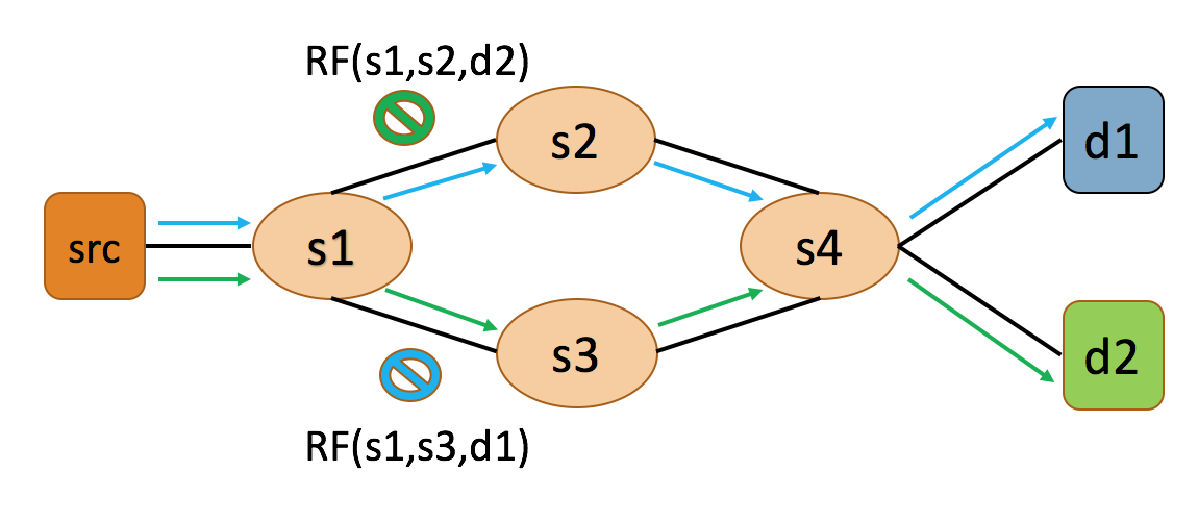
\includegraphics[width=0.7\columnwidth]{figures/diamond.eps}
	\caption{Example of paths that requires route-filtering} \label{fig:diamond}
\end{figure}
The sARC synthesis problem does not always admit a solution.
For example, consider the set of paths illustrated in \Cref{fig:diamond}. 
In this example, both the blue and green paths are required to be the unique shortest paths
and, clearly, this is cannot be enforced for any choice of the edge weights.

In this section, we consider ARCs that use more refined mechanisms to
cope with this problem.
One way to synthesize an ARC in the scenario 
given in \Cref{fig:diamond}
is to ``disable'' the edge
$(s1, s3)$ for destination $d1$.
Using this technique, there is only one possible path from $src$ to $d1$ and the
edge weights become irrelevant for destination $d1$.


This blocking mechanism supported by (non-simplified)
ARC is called a route-filter. 
A route-filter  can selectively disable an
edge for a given destination by  blocking advertisements to a
particular destination along a link. 
Formally, a route-filter is a pair $(l,d)\in L\times S$
disabling a link $l$ for destination $d$
and path to a destination $d$ is \emph{unfiltered} 
if it does not contain edges that are filtered for destination $d$.
%Therefore, if a route-filter is added on switch $s3$, 
%$s3$ 
%will not advertise a route for $d1$ to $s1$, so 
%$s1$ will forward to $s2$ and not to $s3$
%to reach $d1$. The forwarding of packets destined
%for $d2$ are not affected, and they will be sent from
%$s1$ to $s4$ via $s3$ as it is the shortest path.
%Thus, by incorporating route-filters, we can
%disable certain links in the topology 
%for specific destinations, and synthesize
%ARCs for all possible data planes. 
The \emph{ARC synthesis} problem
is to find rational weights for the edges in $L$
and a set of route-filters $F\subseteq L\times S$
 such that 
for each pair of endpoints $(s,t) \in \Gamma$, 
the paths in $P(s,t)$ are the shortest \emph{unfiltered} paths from $s$ to $t$ 
in the graph. 

The ARC synthesis problem admits a trivial solution in which 
route-filters are used to enforce the exact set of input paths by blocking all other possible paths.
This can be done by creating a 
route-filter $(l,d)$ for every link $l$ not in $\xi_d$. 
However, this solution may overly restrict the structure of the network.
In particular, if two nodes were connected by a single path,
a link failure would immediately result in the network becoming disconnected!
Moreover, installing so many route-filters might be costly as not all switches might
support this mechanism.

Ideally, we would like to impose further restrictions to the ARC
synthesis problem to make sure that the obtained solution
satisfy desirable connectivity or resilience properties.
In the following we informally use the word objective 
to identify a property we desire for the synthesized ARC.
Examples of objectives are minimizing the number of route-filters
or maximizing the number of edge-disjoint paths in the ARC
for each endpoint. 
Given an objective $O$, the \emph{augmented ARC synthesis} problem
is to find rational weights for the edges in $L$
and a set of route-filters $F\subseteq L\times S$
 such that 
1) for each pair of endpoints $(s,t) \in \Gamma$, 
the paths in $P(s,t)$ are the shortest \emph{unfiltered} paths from $s$ to $t$ 
in the graph,
2) the resulting ARC satisfies the objective $O$. 
In the following we only allow route-filters for a destination $d$ to be applied to edges of $T$ that are directly connected to 
nodes in $\xi_d$. 

We propose an iterative approach to this problem. 
Our algorithm starts by trying to synthesize a solution
that does not use route-filters using the equations proposed in \secref{sec:sarc}. 
In the case of a failure, the algorithm uses the ``proof of unsatisfiability'' generated by the constraint solver 
to greedily add a small set of route-filters. New equations are then generated and approach is repeated until a solution is found.
We first describe the 
modified linear equations generated when a set of
route-filters are enabled, and then describe two
techniques used to choose route-filters. 
%\begin{figure}
%	\centering
%	\includegraphics[width=\columnwidth]{figures/arcSynthesis.eps}
%	\caption{Synthesis of ARC with route-filters.} \label{fig:arcSynthesis}
%\end{figure}

\minisection{Equations with route-filters}
We show how the technique used to solve the simplified synthesis
problem can be modified to handle filtered and unfiltered paths.
We assume we are given a set of route-filters $F$ and 
use $s\rightarrow_d^* t$ to denote that $s$ can reach $t$
in $T$ without using any edge $l$, such that $(l,d)\in F$.
We use $D_d(sw_1, sw_2)$ to denote the shortest distance from $sw_1$ to $sw_2$
using only edges that are not filtered for destination $d$.
We can revise the equation in \eqref{eq:dist} to correctly restrict the values of $D_d$
by simply ignoring all the filtered edges. 
In the same way, we can modify equations  \eqref{eq:uniq1} and \eqref{eq:uniq2}, while
equation \eqref{eq:uniq3} remains unchanged.

Unfortunately, if the encoding without route-filters produces $n$ equations, this encoding produces $|\Omega|n$ due
to the multiple different distances $D_d$.
Notice that, the shortest distance $D_d(s,t)$ between two nodes $s$ and $t$ without using edges filtered for $d$ cannot be
smaller than the shortest distance $D(s,t)$ obtained without considering route-filters.
We use this property to simplify the encoding by only computing $D(s,t)$ and by replacing each instance of $D_d(s,t)$
with $D(s,t)$ in
equations \eqref{eq:uniq1} and \eqref{eq:uniq2}. 
It is easy to see that every solution of this simplified set of constraints
is also a solution to the original solution (because $D(s,t)\leq D_d(s,t)$).
However, the reverse is not true and the set of simplified equations can be unsatisfiable
in cases in which the original set is satisfiable.
We use the simplified
set of equations in our preliminary implementation and show how it yields encouraging results in practice.

If the set of linear equations does not admit a solution, we 
can add new route-filters so that the equations resulting from the added
route-filters admit a solution.
We discuss two schemes used to add route-filters:
the first scheme uses unsatisfiable cores generated
by the solver and the second scheme 
finds geometrical structures called diamonds that 
cannot be handled without route-filters.


% While detecting diamonds is efficient, the
% presence of diamonds is a not 
% necessary condition for route-filtering.
% Characterising the properties of data planes for which there is
% a pure ARC solution (i.e., no route-filters
% required) is a open algorithmic
% problem. An 
% efficient algorithm to find the structures causing 
% inconsistencies based on these properties 
% can be used to minimize the number of route-filters enabled.  

\minisection{Adding filters using unsatisfiable cores}
Modern LP-solvers have efficient procedures to return an
unsatisfiable core, also called IIS (Irreducible Inconsistent Subsystem)
~\cite{chinneck2007feasibility}. Formally, an IIS is a subset of constraints such that,
if all constraints except those in the IIS are removed, the resulting set of
linear equations is still inconsistent (unsatisfiable). Moreover, the set is irreducible---i.e., removing 
any one constraint of the IIS produces a consistent set of constraints. 

Suppose that, upon producing our set of linear equations, the solver returns unsatisfiable and produces
a concrete unsatisfiable core. 
Some of the linear inequalities from 
Equations \eqref{eq:uniq1} and  \eqref{eq:uniq2}
will appear in the unsat-core 
(an unsat-core cannot consist of only 
constraints from \Cref{eq:dist} and \eqref{eq:uniq3}, as all distances and edges set to zero
would trivially be consistent with these constraints). 
In particular, the unsat-core contains some constraint
\begin{eqnarray}
E(s, n') + D(n', t) > \sum_{\mathclap{\substack{l_i=(s_i,t_i)}}} 
		E(s_i, t_i) 
\end{eqnarray}
that was added to reason about some DAG $\xi_d$.

By adding the route-filter $((s,n'),d)$ to $F$, this inequality is removed from the set of constraints
and the combination of the other constraints appearing in the other unsat-core is now satisfiable.
The complete set of equations may still be inconsistent as other unsat-cores might exist. 
The procedure can be repeated until the resulting set of constraints becomes satisfiable
and we have therefore reached a solution to the ARC synthesis problem.
%\loris{not sure the next paragraph is needed}
%For a given unsat-core, there may be multiple ways to place a route
%filter to eliminate one constraint and we have not investigated
%We can 
%adopt a greedy approach (based on set cover \cite{setcover}) 
%of picking a route-filter which 
%eliminates the maximum number of unsat-cores. However, 
%finding the number of unsat-cores a route-filter eliminates
%is an open problem and instrumental in minimizing the number 
%of route-filters. Other schemes can be used to choose 
%a route-filter from an unsat-core satisfying certain
%objectives. 


\minisection{Diamond elimination}
Finding an IIS is an NP-hard problem~\cite{iiscomplexity}
and can result in slow synthesis times.
We identify a topological property of the set of input paths that 
is guaranteed to require route-filters and use it to produce an initial set of necessary route-filters.
This technique allows us to reduce the number of times we are required to compute  unsat-cores.

We define the structure shown in \Cref{fig:diamond}
as a \emph{diamond}. 
Formally, a problem instance contains a diamond iff there exists two different destinations $d$ and $d'$
such that, in their corresponding DAGs $\xi_d$ and $\xi_{d'}$,
there exists two nodes $s$ and $t$, such that $s\rightarrow_{\xi_d} t$,
$s\rightarrow_{\xi_{d'}} t$, and
there exists a path $l_0\cdots l_n$ from $s$ to $t$ in $\xi_d$ that is not a path from
$s$ to $t$ in $\xi_{d'}$.
As we mentioned at the beginning, synthesizing an ARC for  diamond structures requires
the addition of a route-filter.
In fact, each such a diamond can be ``removed'' by introducing a route-filter $(l_0, d')$ that hides
the path $l_0\cdots l_n$ for the destination $d'$ (see \Cref{fig:diamond}).
Diamonds can detected and removed in polynomial time.

\begin{figure}
	\centering
	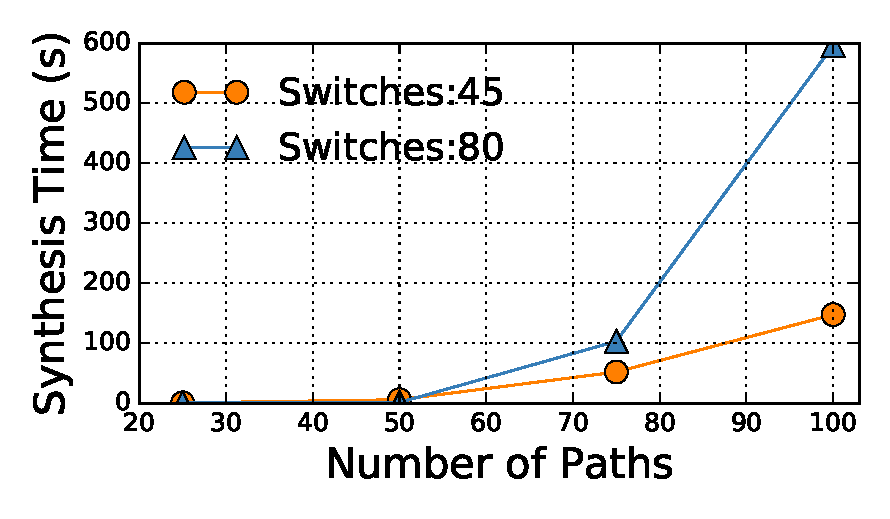
\includegraphics[width=0.7\columnwidth]{figures/evaluation.eps}
	\caption{Preliminary evaluation of synthesis of ARC with
	route-filters.} \label{fig:evaluation}
\end{figure}
\minisection{Evaluation} \Cref{fig:evaluation} shows 
the preliminary evaluation of our second phase, synthesis 
of the ARC with route-filters from the input data plane 
for varying number of paths in the data plane and size 
of a fat-tree topology~\cite{fattree}. 
We generate the input paths randomly
(the maximum path is 7) and report the average 
synthesis time. Our implementation uses the Gurobi 
LP-solver~\cite{gurobi}. 
%
%Consider
%the diamond in \Cref{fig:diamond}. There are two choices
%of route-filters: the $s1-s3$ edge for destination $d1$ 
%and the $s1-s2$ edge for destination $d2$, out of which,
%at least one filter is required to eliminate the 
%inconsistency in the linear equations caused due to the diamond.
%Thus, we find all diamonds for all pairs of destination
%DAGs (this is done in polynomial time) and assign a filter
%to one of the two edges at the source of each diamond. 
%Thus, by removing the diamonds, we can reduce the 
%number of iterations
%of the unsat-core learning approach, which would have 
%provided diamonds as an unsat-core if 
%diamonds were not eliminated.





\subsection{Handling Failures Gracefully}

Another network management consideration for operators is the
occurence of failures (switches, links etc.), which are all too
frequent in datacenter networks~\cite{datacenterfailures}. Failures require
recomputation of paths compliant to the input policies
for the modified topology.  A naive approach is to use \name to
resynthesize the modified instance; However, the new solution may be
drastically different from the original data plane, incurring a large
overhead of removing old rules and installing new
ones~\cite{sdnlatency,updatescheduling}. 
%which could lead to serious
%disruption of tenants' flows.


In what follows, we describe two techniques to handle failures more
gracefully. The first technique is data-plane resiliency (\secref{sec:resiliency}),
which synthesizes and
pre-installs resilient data planes, which even in the event of a
bounded number of link failures, continue to satisfy input
policies. This technique eliminates the need to resynthesize the
forwarding rules for every network failure event, but it 
requires extra backup rules on switches, and it also cannot
capture global operator policies.

Thus, we propose a second mechanism called \emph{minimal repair} (\secref{sec:repair}),
which can transition from the disrupted data
plane to a new policy-compliant one with minimal overhead
 by minimizing the number of
switches whose rule tables are modified. 
Repair does not incur the extra rule cost of the first approach 
and can capture all \Name policies. It is also useful for 
accommodating incremental policy changes, which occur frequently in
cloud datacenters~\cite{mpa-imc15}. The main drawback is that it still
requires removal/installation of rules when a failure occurs, which
can end up being expensive depending on the number of switches
involved.

%% Although the minimal repair mechanism

%% The minimal repair mechanism has two drawbacks: (1) It is {\em reactive}. (2) MaxSMT can be slow to compute a solution impose a high delay to respond to a failure. 
%% cases impose an undue {\em time} overhead in transitioning to the new
%% dataplane.
%% For the new set of policies,
%% \name can use repair to synthesize a new data plane with minimal
%% overhead of installation.



%\name is provided the policies
%and the current forwarding rules $(\overline{Fwd})$ as input. The policy constraints are added as hard
%constraints as described in the earlier sections. To maximize the number of unchanged
%switches, we add \emph{soft} constraints for each switch $sw_1$ of uniform weight as follows:
%Thus, the new forwarding rules $Fwd$ will maximise the number of unchanged
%switch rules in $\overline{Fwd}$, because the constraint will be unsatisfied if a rule on the
%switch changes. 


\subsubsection{Dataplane Resiliency}
\label{sec:resiliency}

%% , and it is crucial to provide
%% certain guarantees during failure scenarios. For example, if the
%% operator wants to guarantee reachability amongst a pair of endpoints,
%% the controller only has to find an active path in the network to
%% re-establish reachability.  However, upon the failure of a link, {\em
%%   reactively} synthesizing a new data plane which satisfies all input
%% policies can be time-consuming, and during this period multiple
%% tenants can suffer from lack of reachability and/or performance
%% issues.  Thus, we propose \emph{policy-compliant resiliency} to tackle
%% network failures by \emph{proactively} synthesizing resilient data
%% planes that even in the event of a bounded number of link failures,
%% continue to satisfy input policies. This eliminates the need to
%% resynthesize the forwarding rules for every network failure event.

In this section, we describe the transformation of input policies to
provide dataplane \emph{t-resilience}~\cite{plinko}, i.e., in the event of
upto $t$ arbitrary link failures, the synthesized data plane still has
a path for each packet class satisfying all policies which is achieved
by synthesizing backup paths that satisfy input policies.  We only
consider reachability, waypoint, and isolation policies in the input.
Global policies like capacity policies and traffic engineering pose a
difficulty in synthesis. For example, consider a packet class $pc$
with a traffic rate of $\sigma(pc)$. By considering the backup paths
with the same traffic characteristics for synthesis, the total traffic
accounted for $pc$ would be $c\times \sigma(pc)$ (for some constant
$c$), leading to under-provisioning of resources. Our current
resilience transformation has no provisions to avoid or minimize the
under-provisioning of resources which affect capacity policies and TE
objectives.
%all backup paths in consideration, while all backup paths will not 
%exist together in the network (backup paths will be deployed during
%a failure event).
%\loris{don't understand previous sentence} \kausik{Have to think!}

Given the physical topology $T=(S,L)$, we define a link-failure
scenario $\theta$ as the set of failed links such that $\theta \subseteq L$.
% For \emph{t-resilience}, we need to
%consider synthesis under any set of $t$ or less arbitrary link failures.
%\begin{mydef}
	We define $\Theta(t)$ as the set of all failure scenarios where no more than $t$
	arbitrary links fail,---i.e. $\Theta(t) = \{ \ \theta \ \ | \ \ |\theta| \leq t\}$.
%\end{mydef}
%We define the projected topology $T^{\theta} = (S, L - \theta)$ as the active 
%physical topology under the failure scenario $\theta$. 	For each class $pc$,
%we construct a data plane graph $\xi = (S, L_{pc})$ for packet class $pc$ from the set
%of paths obtained from the synthesis algorithm. $\xi$
%for class $pc$ over a projected topology $T^\theta$ 
%is resilient if the graph $(S, L_{pc} - \theta)$ has a path from $src$ to $dst$ 
%for the packet class. 
Given a packet class $pc$,
we construct the induced data plane graph $\xi = (S, L_{pc})$ from the links
of the paths returned by the synthesis algorithm for class $pc$.
 For a failure scenario
$\theta$, the active data plane $\xi_\theta = (S, L_{pc} \setminus \theta)$ represents
all the links used by $\xi$ which are unaffected by the failure scenario. A data
plane $\xi$ is {\em resilient} to $\theta$ if it contains a path from the source to 
destination for the packet class in the active data plane $\xi_\theta$.
\begin{mydef}[Resilience]
	A data plane $\xi = (S, L_{pc})$ for class $pc$ is t-resilient if $\xi$ is 
	resilient to all $\theta \in \Theta(t)$.
\end{mydef}
While resilience deals with 
existence of paths during failure scenarios,
we extend the notion to include policy compliance.
\begin{mydef}[Policy-compliance]
	A t-resilient data plane $\xi = (S, L_{pc})$ for class $pc$ is policy-complaint if under
	any failure scenario $\theta \in \Theta(t)$, any path for $pc$ in 
	$\xi_\theta=(S, L_{pc} \setminus \theta)$ satisfies the input policies. 
\end{mydef}
\begin{algorithm}[h]
	\begin{footnotesize}
		\caption{Resilience Transformation}
		\label{restransform}
		\begin{algorithmic}[1]
			\State{[Input] $PC$: Packet classes (Reachability/Waypoint policies)}
			\State{[Input] $I$: Isolation policies (Traffic and Link types)}
			\State{[Input] $t$: Maximum number of arbitrary link failures}
			\State{[Output] $PC^R, I^R$: Transformed set of policies such that the synthesized data
				plane is \emph{t-resilient} and policy-compliant}
			\vspace*{0.25cm}
			\State{$PC^R, I^R \leftarrow \emptyset$}
			\For{$pc:\{src_{pc},dst_{pc},W_{pc}\} \in PC$} 
			\State{// Create $t+1$ edge-disjoint paths of $pc$}
			\State{$\hat{pc} = \{rc_1, rc_2, \ldots rc_{t+1}$\} s.t $\forall m. \ rc_m: \{src_{pc},dst_{pc},W_{pc}\}$} \label{lst:line:respc}
			\State{$PC^R = PC^R \cup \hat{pc}$} 
			\State{$I_{pc} = \{rc_m <> rc_n\ |\ \forall m,n \leq t+1 \wedge m < n\}$}  \label{lst:line:respcisolate}
			\State{$I^R = I^R \cup I_{pc}$} \label{lst:line:respcend}
			\EndFor
			\For{$i: pc_m <op> pc_n \in I$} 
			\State{$\hat{i} = \{ rc_1 <op> rc_2\ | \ \forall rc_1 \in \hat{pc_m}, \forall rc_2 \in \hat{pc_n} \}$} \label{lst:line:respolicy}
			\State{$I^R = I^R \cup \hat{i} $}
			\EndFor \\
			\Return{$PC^R, I^R$}
		\end{algorithmic}
	\end{footnotesize}
\end{algorithm}

\Cref{restransform} shows how \Name can be used to provide \emph{t-resilience}.
The idea is to modify the input policies such that multiple disjoint paths satisfying the original
policies are synthesized for each packet class. 
For \emph{t-resilience}, a packet class $pc$ needs at least $t+1$ edge-disjoint paths from
source to destination. 
We ensure this property holds by creating 
$t+1$ new packet classes ($\hat{pc}$ in line~\ref{lst:line:respc})
and use {\em link-isolation policies} amongst all pairs in $\hat{pc}$ (line \ref{lst:line:respcisolate})
to create $t+1$ edge-disjoint paths for $pc$.
The synthesized data plane $\hat{\xi} = (S, L_{pc})$ for class $pc$ is constructed from the 
paths in the resilient packet class set $\hat{pc} = \{rc_1,\ldots,rc_{t+1}\}$,
i.e., $L_{pc} = \bigcup\limits_{rc \in \hat{pc}} L_{rc}$.  
Each path of $\hat{pc}$ satisfies the reachability policy, 
and any arbitrary $t$ link failure scenario cannot affect all $t+1$ paths.

However, the resilient paths need to satisfy the input isolation policies with other 
packet classes (which themselves have $t+1$ paths for resilience). Thus, for a 
given policy $pc_1 || ~pc_2$, we add isolation policies to every pair of 
classes of $\hat{pc_1}$ and $\hat{pc_2}$ (line \ref{lst:line:respolicy}). This ensures that any path 
chosen in the data planes of $pc_1$ and $pc_2$ will be isolated from one 
another, thus providing policy-compliance under any arbitrary $t-link$ failure
scenario. \Cref{fig:restransform}(a) demonstrates an example transformation for providing $1-resilience$. 

\noindent We now that \Cref{restransform} is sound.
\begin{theorem}[Soundness]
Given input policies $(PC, I)$, 
the data plane $\hat{\xi}_{pc}$ for every packet class $pc \in PC$
 synthesized from
transformed policies $(PC^R, I^R)$  is \emph{t-resilient} 
	and policy-compliant. 
\end{theorem}
\iffull
\begin{proof}
		Assume, $\exists pc$ such that the data plane $\hat{\xi} = (S, L_{pc})$
		is not \emph{t-resilient}. 
		Therefore, there exists a failure scenario $\theta$ such that $|\theta| \leq t$ 
		and $\hat{\xi}_\theta = (S, L_{pc} \setminus \theta)$ 
		is not resilient, i.e., there is no path from the source to destination. 
		Thus, $\theta$ disabled all the paths of $\hat{pc}$. \\
		However, the paths are
		edge-disjoint as each class in $\hat{pc}$ has a link-isolation policy with each 
		other. Thus, $t$ link failures cannot affect $t+1$ 
		edge-disjoint paths of $\hat{pc}$. Thus, $\theta$ disabling all paths of
		$\hat{pc}$ is a contradiction. \\
		Let us consider policy-compliance. Given a failure scenario $\theta \in \Theta(t)$, each data plane $\xi$ of class $pc$ has an active path. Consider a isolation policy in $I$: $pc_1 || \ pc_2$. In line~\ref{lst:line:respolicy} of \Cref{restransform}, each class of $\hat{pc_1}$ will be isolated to
		each class of $\hat{pc_2}$, thus any path of the data planes of $pc_1$ and
		$pc_2$ will satisfy the input policy $pc_1 || \ pc_2$. Hence, the data planes 
		are policy-compliant. 
	\end{proof}
	\fi
\noindent If there are no isolation policies in the input, the resilience transformation in lines 
\ref{lst:line:respc}-\ref{lst:line:respcend} of \Cref{restransform} is complete.
\begin{theorem}[Completeness]
%\loris{What is the input? You should say.
%Given .... such that ...., the synthesized data plane... is....if and only if...}
Given input policies $(PC,I)$ such that $I=\emptyset$,
the synthesized data plane $\xi$ for a packet class $pc$  
is \emph{t-resilient} if and only if it 
contains $t + 1$ edge-disjoint paths from source to destination
for $pc$.
%If there are no isolation policies $I = \emptyset$, 
%	for a packet classes $pc$, the data plane \loris{what dataplane?} is \emph{t-resilient} only if it 
%	contains $t + 1$ edge-disjoint paths for $pc$.
\end{theorem}
\iffull
	\begin{proof}
		We have proved the soundness of the result in \Cref{resiliencesoundness}. 
		Now, let us assume the data-plane $\hat{\xi}$ for $pc$ is \emph{t-resilient} such 
		that less than $t+1$ instances of $pc$ are required for resilience i.e. 
		$|\hat{pc}| < t+1$. Let us consider a 
		t-link failure scenario $\theta, |\theta| = t$ where a link is picked from
		each path of $\hat{pc}$. The active data plane
		$\hat{\xi}_\theta = (S, L_{pc} \setminus \theta)$ will not contain a
		path from source to destination as all paths of $\hat{pc}$ would be disabled.  
		This is a contradiction since $\hat{\xi}$ is \emph{t-resilient}. 
		Therefore, we need atleast $t+1$ instances of $pc$ to ensure \emph{t-resilience}.
		
		Now let us assume there are $t+1$ paths in a \emph{t-resilient} $\hat{\xi}$ for $pc$,
		and not all of them are edge-disjoint. Consider two paths $\pi_1$ and $\pi_2$
		in $\hat{\xi}$ which share a link. We can choose the shared link 
		of $\pi_1$ and $\pi_2$ and $t-1$ links from the other $t-1$ paths 
		and construct a failure scenario $\theta$, $|\theta| = t$.
		The active data plane
		$\hat{\xi}_\theta = (S, L_{pc} \setminus \theta)$ will not contain a
		path from source to destination as all paths of $\hat{pc}$ would be disabled.  
		This is a contradiction since $\xi$ is \emph{t-resilient}. Therefore,
		the $t+1$ paths of $pc$ must be edge-disjoint. 
		
		\noindent Thus, the resilience transformation is sound and complete for a  
		packet class if there are no isolation policies.
	\end{proof}
\fi

%\noindent The transformation demonstrated in \Cref{restransform} is not \emph{complete}
% if the original policies contain link-isolation policies i.e. if the transformed policies
% are unsatisfiable, 
% that does not imply the non-existence of resilient data planes. 
When the original policies contain link-isolation policies, the policies
from \Cref{restransform} may return \texttt{unsat} even when a
resilient data plane exists. Specifically, line~\ref{lst:line:respolicy}
can add additional policies than is required for resilience.
% This is because link-isolation causes edge-disjointness of paths,
% and thus, cannot be both affected by a link failure. 
 \Cref{fig:restransform}(b) shows a transformation required for $1-resilience$ 
 with a smaller number of link-isolation policies among different classes
 of $pc_1$ and $pc_2$ than one obtained from \Cref{restransform}. 
 Consider a failure scenario which disables path
 of $pc_{1A}$. By virtue of the link-isolation policies, $pc_{1B}$ and
 $pc_{2A}$ will be unaffected and can be used as paths for $pc_1$ 
 and $pc_2$ respectively, and $pc_1 <> pc_2$ holds. Now suppose
 $pc_{1B}$ is affected. Similarily, $pc_{1A}$ and $pc_{2A}$ can be used as
 the paths for the original packet classes. The same scenarios hold symmetrically
 for $pc_2$, and thus the resilience transformation can be achieved without
 adding link-isolation policies amongst all the packet classes. 
 
\begin{figure}
	\centering
	\subfloat[Traffic Isolation]{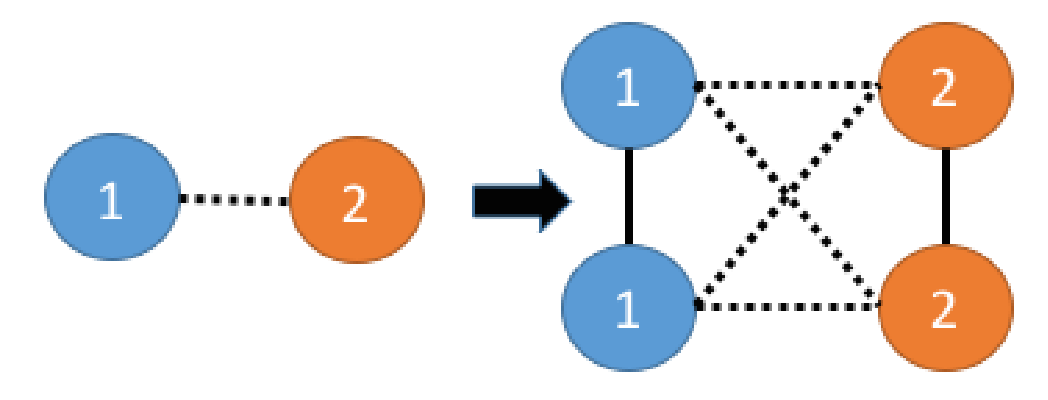
\includegraphics[width=0.5\columnwidth]{figures/resilience.eps}}
	\subfloat[Link Isolation]{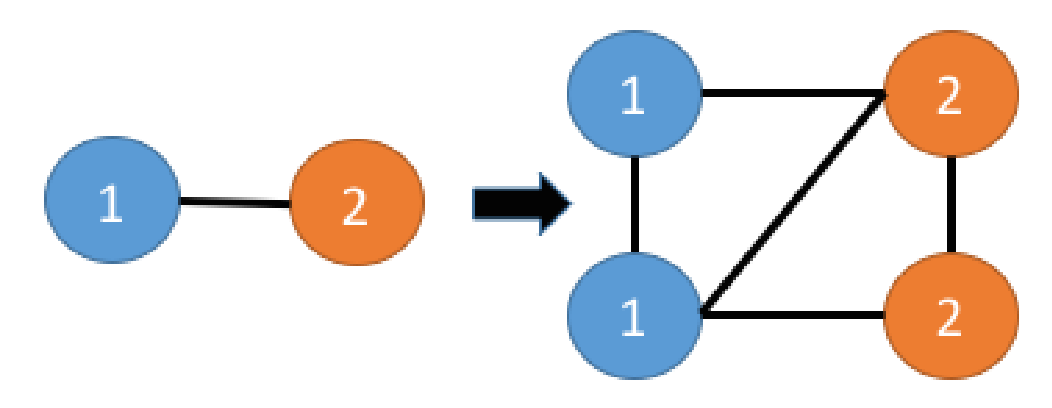
\includegraphics[width=0.5\columnwidth]{figures/resilience-cex.eps}}
	\caption{\label{fig:restransform}
		(a) Resilience Transformation for $pc_1 || \ pc_2$ for providing $1-resilience$. 
		The dotted lines represent traffic isolation policies, 
		while the solid lines represent link isolation. (b) Example of a sufficient transformation
		for 1-resilience in the case of a link-isolation policy.}
\end{figure}

%We presented a sound transformation of policies to provide \emph{t-resilience} in
%the case of reachability, waypoint and isolation policies. Future directions of 
%research involve incorporating capacity constraints and traffic engineering
%for synthesis of resilient data planes and devising a complete transformation for isolation.

\subsubsection{Minimal Repair} \label{sec:repair}
%% Thus, operators need
%% a \emph{network repair} mechanism which can transition with minimal
%% overhead from the current data plane to a policy-compliant one.  This
%% repair mechanism is also useful to accomodate incremental policy
%% changes, which occurs frequently in cloud
%% datacenters~\cite{mpa-imc15}.  For the new set of policies, \name can
%% use repair to synthesize a new data plane with minimal overhead of
%% installation.

Dataplane resiliency imposes high rule storage overhead on switches,
and cannot accommodate global policies like link capacity bounds. 
As an alternative to it, we
extend \name's synthesis algorithm to perform minimal network
repair using MaxSMT.

Formally, the MaxSMT problem is as follows:
given a set of formulas $\Psi_0, \Psi_1, \ldots, \Psi_n$ with
associated weights $w_1, \ldots, w_n$, find a subset $M \subseteq \{1,
\ldots n\}$ s.t:
1) $\Psi_0 \wedge \bigwedge_{i \in M} \Psi_i$ is satisfiable, and 
2) The \emph{award} $\sum_{i \in M} w_i$  is maximized. 
The constraints $\Psi_1, \ldots, \Psi_n$ denote \emph{soft} constraints, and
the associated weights $w_i$ encode the award for including $\Psi_i$ in the satisfying
assignment. 
%The basic intuition is that
%we add the existing configuration as \emph{soft} constraints to the set of \emph{hard} 
%policy constraints. The solver would return a solution which \emph{maximizes} the 
%number of satisfied soft constraints (the older configuration),
%thus resulting in a new policy-compliant forwarding 
%configuration with minimal 
%number of changes from the older one and reducing the overhead of
%updating the forwarding rules in the network.  

We reduce the network repair problem to a MaxSMT problem
and use soft constraints to minimize the number of 
switches on which rules need to be updated. Note that
the disadvantage w.r.t. dataplane resiliency is that switches still
require rule updates, which may take time depending on the number of
switches involved.

 Let the policy constraints generated by \name for the new network
 state be $\Psi_0$, and let $\overline{Fwd}$ be the present data plane
 that does not satisfy $\Psi_0$. The objective is to find new $Fwd$
 which satisfies $\Psi_0$ while maximizing the number of \emph{preserved
   switches} (switches whose rules are unchanged). If the
 rules on switch $sw_i$ are preserved, then $Fwd$ and $\overline{Fwd}$
 have the same forwarding rules for all packet classes which traverse
 through $sw_i$. The following soft constraints capture this idea:
\begin{equation}
	\Psi_{sw_i} =  
	  \bigvee_{\mathclap{\substack{\forall sw_j, pc \\
			  		(sw_i, sw_j, pc) \in \overline{Fwd}}}} Fwd(sw_i, sw_j, pc) 
			~~~~~~~~~~~ 
			w_{sw_i}= 1
\end{equation}
The solution to this MaxSMT problem is a data plane that minimizes the number of
switches whose rules have to be changed.  Alternate repair objectives
like minimizing the number of changed forwarding rules can be
expressed similarly. Interestingly, the \name's network repair
mechanism can also be used to transform an existing
non-compliant data plane to a policy-compliant one.

\subsection{Resilient \ARCs to device configurations}
To deploy the resulting control plane, the \ARC must be
transformed to actual device configurations expressed in a
generic~\cite{openconfig} or vendor-specific~\cite{ciscoios} language. \ARC's
semantics are equivalent to the semantics of OSPF and layer-3 access control
lists (ACLs). Thus, we can trivially compile the \ARC into device
configurations by: (1) setting the OSPF link weights to the edge weights of
the \ARC, and (2) adding a layer-3 ACL for each route-filter in the ARC.
However, the resulting configurations may be overly
complex~\cite{complexitymetrics} or use features that make the network more
prone to failures~\cite{mpa-imc15}. Consequently, part of our future work is to
explore how to generate more optimal configurations from \ARCs.

%\aaron{TODO: talk about the task of generating configurations from an \ARC}
%Gember-Jacobson et al.~\cite{arc} describe the process 
%of generating the \ARC from the device configurations by transforming 
%the concrete network protocol parameters to create weighted digraphs. 
%Our three-phased architecture to synthesize distributed control planes
%from policies produces the \ARC which has to be compiled to 
%individual device configurations, which is the inverse of 
%the process tackled by Gember-Jacobson et al. ~\kausik{something more?}
%
%For example, suppose the underlying network comprises 
%one complete OSPF domain. For this, we can trivially
%compile the \ARC to individual device configurations by: (1)
%setting the OSPF link weights to the edge weights of the \ARC, and
%(2) adding a route-filter or Access Control List (ACL) for the 
%route-filters in the ARC. However, the compilation process becomes
%complicated if the network consists of multiple OSPF 
%domains, and use BGP for intra-domain communication. 

\section{Discussion}

\section{Conclusion}

We presented \Name, a general and extensible network management system
for enterprise-scale multi-tenant datacenter networks. It allows
rich policies to be specified declaratively. It leverages
the formal reasoning foundations of constraint solving together with
fast SMT solvers to synthesize data plane configuration from high
level policies. This abstracts away the difficult of programming or
configuring individual switches. \Name incorporates novel ideas to
speed up synthesis, leveraging the hierarchical nature of datacenter
network topologies and the structure of the interaction between
tenants' policies. These optimizations help \Name synthesize policies
for realistic settings in a few seconds, making it pratical to use in
network management.

%   Operators in multi-tenant cloud data centers require support for
%   diverse and complex end-to-end policies like reachability, middlebox
%   traversals, isolation, and network resource management. We present
%   \Name, a network management system which allows these policies to be
%   specified in a declarative manner without explicitly programming the
%   data-plane behavior.  \name tackles the problem of enforcing the
%   policies by synthesizing switch forwarding tables. In doing so, it
%   uses the formal reasoning foundations of constraint solving in
%   combination with fast off-the-shelf SMT solvers.  To improve
%   synthesis performance, \Name incorporates a novel search strategy that
%   uses regular expressions to specify properties that leverage the
%   structure of datacenter networks,
% %topologies to specify properties of the path 
%   and a heuristic synthesis procedure which exploits the structure of
%   policy interactions.  Experiments demonstrate the performance of
%   \Name with different workloads on real-world topologies. Overall,
%   the approach used by \Name is general and instrumental to building a
%   comprehensive network management system.


\bibliographystyle{abbrv} 
\begin{small}
\bibliography{refs}
\end{small}
\label{last-page}

\end{document}

